% !TeX spellcheck = cs_CZ
%{\tikzset{external/prefix={tikz/FYZI/}}
% \tikzset{external/figure name/.add={ch26_}{}}
%=========================== Kapitola: Optika: Princip nejkratšího času ===========================
\chapter{Optika: Princip nejkratšího času}\label{fyz:IchapXXVI}
\minitoc
  \section{Světlo}\label{fyz:IchapXXVIsecI}
    Začínáme první z několika kapitol na téma \emph{elektromagnetické záření}. Světlo, pomocí něhož 
    vidíme, je jen jednou nepatrnou součástí rozsáhlého spektra jevů stejného druhu. Různé části 
    tohoto spektra se liší různými hodnotami určité proměnné veličiny. Tuto veličinu můžeme nazvat 
    \emph{vlnová délka}. Podle její změny ve viditelném spektru mění světlo svou barvu od červené 
    po fialovou. Zkoumáme-li spektrum systematicky směrem od dlouhých vlnových délek ke kratším, 
    začneme tím, čemu obyčejně říkáme rádiové vlny. Rádiové vlny jsou technicky dostupné v širokém 
    rozsahu vlnových délek a některé jsou dokonce delší než ty, jež se používají při běžném 
    vysílání; běžné vysílače používají vlnovou délku kolem 500 metrů. Dále existují krátké vlny, 
    radarové vlny, pak milimetrové vlny atd. Skutečné hranice mezi jedním rozsahem vlnových délek a 
    druhým rozsahem neexistují, protože příroda nás neobdařuje ostrými rozhraními. Číselné údaje 
    přiřazené jednotlivým názvům vln jsou jenom přibližné a to samozřejmě platí i o názvech, které 
    dáváme různým vlnovým rozsahům. 
    
    Daleko pod milimetrovými vlnami nacházíme \emph{infračervené} vlny a potom viditelné spektrum. 
    Ještě dál se dostaneme do oblasti, jíž říkáme \emph{ultrafialová}. Tam, kde tato oblast končí, 
    začínají rentgenové paprsky, ale kde to přesně je, nemůžeme definovat; je to asi při 
    \SI{e-8}{\m} neboli \SI{e-2}{\micro\m}. To jsou měkké rentgenové paprsky; dále jsou tam 
    normální rentgenové paprsky a velmi tvrdé rentgenové paprsky; dále paprsky gama, a tak můžeme 
    postupovat ke stále menším a menším hodnotám veličiny nazvané vlnová délka.
    
    V tomto obrovském rozsahu vlnových délek se nacházejí tři nebo i více oblastí aproximací, jež 
    jsou zvlášť zajímavé. V jedné z nich platí podmínka, že příslušné vlnové délky jsou velmi malé 
    ve srovnání s rozměry zařízení, jež se používají pro jejich studium; dále, že energie fotonů, 
    použijeme-li kvantovou teorii, jsou malé ve srovnání s energetickou citlivostí zařízení. Za 
    těchto podmínek můžeme udělat první aproximaci pomocí \textbf{geometrické optiky}. Na druhé 
    straně, jsou-li vlnové délky srovnatelné s rozměry zařízení (čehož lze obtížně dosáhnout s 
    viditelným světlem, ale lépe s radiovlnami) a jsou-li energie fotonů stále zanedbatelně malé, 
    lze použít velmi užitečnou aproximaci \textbf{vlnové optiky}, bez přihlédnutí ke kvantové 
    mechanice. Tato metoda se zakládá na klasické teorii elektromagnetického záření, kterou si 
    probereme v některé další kapitole. Přejdeme-li k velmi krátkým vlnám, kde si nemusíme všímat 
    vlnových vlastností a kde fotony mají velkou energii ve srovnání s citlivostí zařízení, celá 
    věc se opět zjednoduší. To je jednoduchá \textbf{fotonová představa}, kterou si popíšeme jen 
    přibližně. Celkový obraz, který všechno spojuje do jednoho modelu, nebudeme mít ještě dlouho k 
    dispozici.
    
    V této kapitole se omezíme na oblast geometrické optiky, v níž zapomeneme na vlnovou délku a na 
    fotonový charakter světla, jímž se budeme zabývat později. Nedáme si dokonce ani tu námahu, 
    abychom řekli, co to je světlo, pouze zjistíme, jak se chová v oblastech mnohem větších než je 
    vlnová délka. Toto všechno je třeba říct, abychom zdůraznili skutečnost, že to, o čem budeme 
    mluvit, je jen hrubá aproximace; je to jedna z kapitol, kterou se budeme muset zase „odnaučit“. 
    Uděláme to však velmi rychle, neboť téměř ihned přejdeme k metodě, jež je přesnější.
    
    I když geometrická optika je jen aproximací, je důležitá pro techniku a historicky je velmi 
    zajímavá. Proto ji budeme prezentovat více historicky, než jiné předměty, abychom si udělali 
    představu o rozvoji fyzikální teorie, fyzikálního názoru.
    
    Světlo je, samozřejmě, každému známé, a tak to bylo od nepaměti. Jedna otázka zní, jak vlastně 
    světlo vidíme. O této problematice existovalo mnoho teorií, které se nakonec shodly na jednom, 
    že totiž existuje něco, co vchází do oka - a vytváří v něm obraz předmětů. Toto vysvětlení jsme 
    slyšeli tak dávno, že ho přijímáme a téměř si nemůžeme představit, že skutečně inteligentní 
    lidé mohli předložit opačné teorie - např. že něco vychází z oka, co „ohmatává“ předměty. Z 
    některých dalších důležitých pozorování vyplývá, že jak světlo letí z místa na místo, pohybuje 
    se přímočaře (pokud mu nic nestojí v cestě) a že světelné paprsky navzájem neinterferují. To 
    znamená, že světlo v místnosti prochází všemi směry, ale světlo, které křižuje směr našeho 
    vidění, neovlivní to světlo, které k nám přichází od nějakého předmětu. To byl kdysi 
    nejsilnější argument proti korpuskulární teorii světla, jejž použil Huygens. Kdyby bylo světlo 
    množstvím souběžně letících šípů, jak by jiné šípy mohly jím tak hladce proniknout? Takové 
    filozofické argumenty však nemají velkou váhu. Můžeme stejně tak tvrdit, že světlo se skládá z 
    šípů, jež se mohou vzájemně pronikat!
    
  \section{Odraz a lom}\label{fyz:IchapXXVIsecII}
    Předcházející diskuze nám dala základní představu o geometrické optice: nyní musíme jít trochu 
    dále ke kvantitativním vlastnostem. Dosud máme jen světlo letící po přímkách mezi dvěma body. 
    Nyní studujme vlastnosti světla, když naráží na různé materiály. Nejednodušším objektem je 
    zrcadlo. Platí pro něj zákon, že narazí-li světlo na zrcadlo, nepokračuje dále po přímce, ale 
    odráží se od zrcadla ve směru jiné přímky, která se mění, měníme-li sklon zrcadla. Otázkou pro 
    lidi ve starověku bylo, jaký je vztah mezi dvěma úhly, jež charakterizují takový odraz. Je to 
    velmi jednoduchý vztah, jenž byl objeven dávno. Světlo dopadající na zrcadlo se odráží takovým 
    způsobem, že oba úhly mezi každým paprskem a zrcadlem jsou stejné. Z nějakých důvodů je zvykem 
    měřit úhly od kolmice k povrchu zrcadla. Vztah nazývaný \textbf{zákon odrazu} má tvar
    \begin{equation}\label{fyz:eq336}
      \alpha_1 = \alpha_1'
    \end{equation}
    
    \begin{figure}[ht!] %\ref{fyz:fig279}
      \centering
      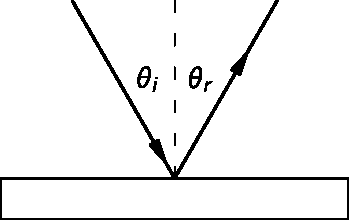
\includegraphics[width=0.5\linewidth]{fyz_fig279.pdf}
      \caption{Úhel dopadu je roven úhlu odrazu
               (\cite[s.~346]{Feynman01})}
      \label{fyz:fig279}
    \end{figure}

    \begin{wraptable}[21]{r}{4cm}      %\ref{fyz:tab007}
      \centering
      \renewcommand{\arraystretch}{1.4}
      \begin{tabular}{>{\centering\arraybackslash}p{3em}|>{\centering\arraybackslash}p{3em}}
         \hline \(\sphericalangle\) & \(\sphericalangle\)     \\
                    vzduch & voda         \\
         \hline   \ang{10} & \ang{8}      \\
                  \ang{20} & \ang{15.5}   \\
                  \ang{30} & \ang{22.5}   \\
                  \ang{40} & \ang{29}     \\
                  \ang{50} & \ang{35}     \\
                  \ang{60} & \ang{40.5}   \\
                  \ang{70} & \ang{45.5}   \\
                  \ang{80} & \ang{50}     \\
         \hline 
      \end{tabular}
      \caption{Ptolemaiovy hodnoty pro lom světla vzduch - voda 
               (\cite[s.~347]{Feynman01})}
      \label{fyz:tab007}
    \end{wraptable}
    To je dostatečně jednoduchá poučka. S větším problémem se však setkáváme při přechodu světla z 
    jednoho prostředí do druhého, například při přechodu ze vzduchu do vody; zde také vidíme, že 
    světlo nepokračuje v pohybu po téže přímce. Ve vodě je paprsek odkloněn od směru své dráhy, 
    kterou měl ve vzduchu. Změníme-li úhel \(\alpha_1\) tak, že paprsek dopadá téměř kolmo, úhel 
    lomu není tak velký, ale když paprsek dopadá pod velkým úhlem, úhel odklonu je velmi velký. 
    Otázkou je, jaký vztah platí mezi těmito úhly? To také dlouho znepokojovalo lidi ve starověku a 
    nikdy na to nenašli odpověď! Klaudios Ptolemaios však sestavil seznam úhlů ve vodě pro různé 
    úhly ve vzduchu. Je to jedno z mála míst z celé řecké fyziky, kde lze najít nějaké 
    experimentální výsledky. V tabulce \ref{fyz:tab007} jsou uvedeny úhly pro vzduch (ve stupních) 
    a jim odpovídající úhly naměřené pro vodu. (Říká se, že řečtí vědci nikdy neprováděli žádné 
    experimenty, ale získat takovou tabulku hodnot bez znalosti správného zákona je možné pouze 
    experimentálně. Je však třeba si všimnout, že tyto hodnoty nepředstavují výsledky nezávislých 
    měření pro každý úhel, ale jen čísla získaná interpolací z několika měření, neboť všechny leží 
    přesně na parabole.)

    \begin{figure}[ht!] %\ref{fyz:fig280}
      \centering
      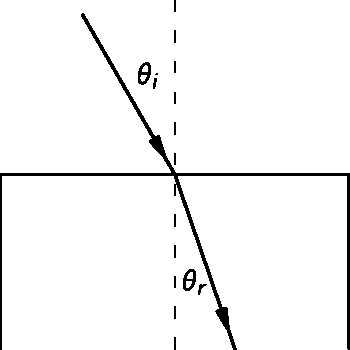
\includegraphics[width=0.5\linewidth]{fyz_fig280.pdf}
      \caption{Světelný paprsek se láme při přechodu z jednoho prostředí do druhého
               (\cite[s.~346]{Feynman01})}
      \label{fyz:fig280}
    \end{figure}
    
    To je tedy jeden z důležitých stupňů ve vývoji fyzikálního zákona: Nejdřív pozorujeme nějaký 
    jev, dále ho měříme a sestavíme si tabulku a potom se pokoušíme najít pravidlo, pomocí něhož
    lze spojit jeden poznatek s druhým. Tabulka \ref{fyz:tab007} byla sestavena v roce 140 n. l., 
    avšak až r. 1621 bylo nalezeno pravidlo spojující tyto dva úhly. Toto pravidlo, objevené 
    holandským matematikem Willebrordem Snellem, zní: \emph{Je-li úhel ve vzduchu \(\alpha_1\) a 
    úhel ve vodě \(\alpha_2\), sinus \(\alpha_1\) je roven néjakému konstantnímu násobku sinu 
    \(\alpha_2\)}
    \begin{equation}\label{fyz:eq337}
      \sin\alpha_1 = n\cdot\sin\alpha_2
    \end{equation}
    
    Číslo \(n\) je pro vodu přibližně \num{1.33}. Rovnice (\ref{fyz:eq337}) se nazývá 
    \textbf{Snellův zákon}. Dovoluje nám předpovědět, jak se světlo láme při přechodu ze vzduchu do 
    vody. Tabulka \ref{fyz:tab008} uvádí úhly ve vzduchu a ve vodě podle Snellova zákona. Všimněte 
    si pozoruhodné shody s Ptolemaiovými hodnotami.

    \begin{table}[ht!]     %\ref{fyz:tab008}
      \centering
      \renewcommand{\arraystretch}{1.4}
      \begin{tabular}{>{\centering\arraybackslash}p{3em}|>{\centering\arraybackslash}p{3em}}
         \hline \(\sphericalangle\) & \(\sphericalangle\)     \\
                    vzduch & voda         \\
         \hline   \ang{10} & \ang{7.5}    \\
                  \ang{20} & \ang{15}     \\
                  \ang{30} & \ang{22}     \\
                  \ang{40} & \ang{29}     \\
                  \ang{50} & \ang{35}     \\
                  \ang{60} & \ang{40.5}   \\
                  \ang{70} & \ang{45}     \\
                  \ang{80} & \ang{48}     \\
         \hline 
      \end{tabular}
      \caption{Úhly ve vzduchu a ve vodě podle Snellova zákona lomu.
               (\cite[s.~347]{Feynman01})}
      \label{fyz:tab008}
    \end{table}
    
  \section{Fermatův princip nekratšího času}\label{fyz:IchapXXVIsecIII}
    Při dalším rozvíjení vědy chceme víc než jen matematickou formuli. Nejdříve máme pozorování, 
    pak čísla, jež jsme naměřili, potom máme zákon, jenž sumarizuje všechna tato čísla. Velkou 
    předností vědy je však to, že jsme schopni najít takový způsob uvažování, kdy se zákon stává 
    zřejmým. 
    
    První způsob uvažování, ze kterého zákon šíření světla vyplynul jako zřejmý, objevil Fermat 
    kolem r. 1650 a nazývá se \emph{princip nejkratšího času} nebo \textbf{Fermatův princip}. 
    Spočívá v tom, že ze všech možných drah, kterými se lze dostat z jednoho bodu do druhého, si 
    světlo vybírá takovou, která vyžaduje nejkratší čas. 

    \begin{figure}[ht!] %\ref{fyz:fig281}
      \centering
      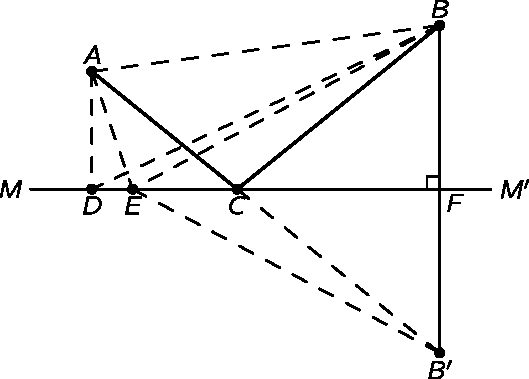
\includegraphics[width=0.8\linewidth]{fyz_fig281.pdf}
      \caption{Znázornění principu nejkratšího času
               (\cite[s.~348]{Feynman01})}
      \label{fyz:fig281}
    \end{figure}
    
    Nejprve si ukážeme platnost principu pro zrcadlo. Zjistíme, že tento jednoduchý princip 
    obsahuje oboje - zákon přímočarého šíření i zákon pro zrcadlo. (Naše chápání se prohlubuje!) 
    Pokusme se najít řešení následujícího problému. Na obrázku \ref{fyz:fig281} jsou znázorněny 
    body \(A\) a \(B\) a rovinné zrcadlo \(MM'\). Jakou cestou je možné se dostat z \(A\) do \(B\) 
    za nejkratší čas? Odpověď: přímo z \(A\) do \(B\)! Když ale přidáme další podmínku, že světlo 
    se musí odrazit od zrcadla a vrátit se zpět za co nejkratší dobu, odpověď není tak snadná. 
    Jeden způsob by byl, co nejdříve dorazit k zrcadlu a pak do bodu \(B\) - po dráze \(ADB\). 
    Potom máme samozřejmě dráhu \(DB\) dlouhou. Přesuneme-li se o málo doprava do bodu E zvětšíme 
    si o něco první vzdálenost, ale druhou si velmi zkrátíme, takže celková délka dráhy, a tedy i 
    čas potřebný k jejímu překonání jsou kratší. Jak lze najít bod \(C\), pro nějž je čas 
    nejkratší? Velmi jednoduše ho můžeme najít pomocí geometrického triku.
    
    Na druhé straně roviny \(MM'\) sestrojíme pomocný bod \(B'\), jenž se nachází stejně daleko pod 
    rovinou \(MM'\) jako bod \(B\) nad touto rovinou a nakreslíme úsečku \(EB'\). Protože úhel 
    \(BFM\) je pravý a \(BF = FB'\), i \(EB\) je rovno \(EB'\). Součet vzdáleností \(AE + EB\), 
    úměrný času, který vyžaduje světlo pohybující se konstantní rychlostí, bude roven součtu 
    vzdáleností \(AE + EB'\). Otázkou tedy je, kdy je součet těchto dvou vzdáleností nejmenší. 
    Odpověd je jednoduchá: Tehdy, když čára prochází bodem \(C\) jako přímka z \(A\) do \(B'\)! 
    Jinými slovy, je třeba najít bod, přes nějž se dostaneme do pomocného bodu \(B'\), a to bude 
    ten správný bod. Je-li \(ACB'\) přímka, pak úhel \(BCF\) je roven úhlu \(B'CF\) a tedy i úhlu 
    \(ACM\). Výrok, že úhel dopadu je roven úhlu odrazu, je tedy ekvivalentní výroku, že světlo 
    dopadá na zrcadlo tak, že do bodu \(B\) se vrací za \emph{nejkratší možný čas}. Autorem 
    původního výroku, že světlo se šíří tak, že k zrcadlu a pak k jinému bodu jde po nejkratší 
    možné dráze, je Heron Alexandrijský, není to tedy moderní teorie. Inspirovala však Fermata k 
    myšlence, že i lom světla probíhá na témž základě. Ale při lomu světla je jasné, že světlo 
    nejde po nejkratší vzdálenosti, proto Fermat přišel na myšlenku, že to bude za \emph{nejkratší 
    čas}.
    
    \begin{figure}[ht!] %\ref{fyz:fig282}
      \centering
      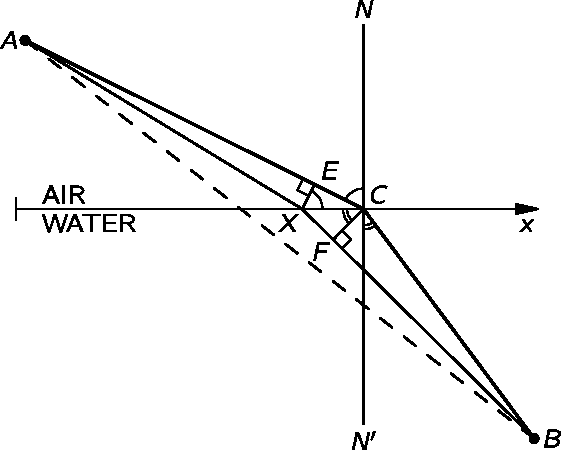
\includegraphics[width=0.8\linewidth]{fyz_fig282.pdf}
      \caption{Znázornění Fermatova principu pro lom světla
               (\cite[s.~348]{Feynman01})}
      \label{fyz:fig282}
    \end{figure}

    Dříve, než se pustíme do analýzy lomu světla, měli bychom udělat ještě jednu poznámku o 
    zrcadle. Máme-li v bodě \(B\) zdroj, jenž vysílá světlo směrem k zrcadlu, vidíme, že světlo, 
    přichází z bodu \(B\) do bodu \(A\) přesně tak, jakoby vycházelo z bodu \(B'\) a neměli bychom 
    žádné zrcadlo. Samozřejmě, oko registruje jen to světlo, které do něho vnikne, takže, máme-li 
    nějaký předmět v bodě \(B\) a zrcadlo, jež způsobuje, že světlo nám vnikne do oka přesně 
    stejně, jako by vnikalo do oka, kdyby byl předmět v bodě \(B'\), systém oko - mozek to 
    interpretuje tak (za předpokladu, že o tom mnoho neví), že předmět je v bodě \(B'\). Dojem, že 
    předmět se nachází za zrcadlem, vzniká jenom proto, že světlo, jež vniká do oka, vniká do něho 
    fyzikálně přesně stejně, jako by vnikalo z předmětu umístěného za zrcadlem (odhlédneme-li od 
    nečistoty na zrcadle, od toho, že víme o existenci zrcadla atd., což se v mozku koriguje).
    
    Nyní ukažme, že z principu nejkratšího času vyplývá Snellův zákon lomu. Musíme však formulovat 
    předpoklad o rychlosti světla ve vodě. Budeme předpokládat, že rychlost světla ve vodě je 
    \(n\)-krát menší než rychlost světla ve vzduchu.
    
    Na obrázku \ref{fyz:fig282} máme opět problém, jak se dostat z \(A\) do \(B\) za nejkratší čas. 
    Abychom ukázali, že nejlepší, co lze udělat, není postupovat po přímce, představme si, že v 
    bodě \(B\) vypadlo z člunu do vody pěkné děvče a volá o pomoc. Čára označená jako \(x\) je 
    břeh. My se nacházíme v bodě \(A\) na zemi, vidíme, co se stalo a umíme běhat i plavat, ale 
    běhat umíme rychleji než plavat. Co uděláme? Půjdeme přímo? (Ano, bez pochyb!) Avšak, při troše 
    větší inteligence, bychom si uvědomili, že by bylo výhodné projít o něco více po zemi, abychom 
    si zkrátili vzdálenost po vodě, neboť pohyb ve vodě je mnohem pomalejší. Podle tohoto způsobu 
    uvažování bychom řekli, že nejsprávnější by bylo napřed přesně vypočítat, jak máme běžet. V 
    každém případě se pokusme ukázat, že konečným řešením problému je dráha \(ACB\), jíž odpovídá 
    nejkratší možný čas. Z toho, že je to nejkratší čas, vyplývá, že zvolíme-li si jakoukoliv jinou 
    dráhu, čas na její absolvování bude delší. Kdybychom si tedy graficky znázornili potřebný čas v 
    závislosti na poloze bodu \(X\), dostali bychom křivku podobnou křivce na obr. 
    \ref{fyz:fig283}, kde bod \(C\) odpovídá nejkratšímu ze všech možných časů. Vidíme, že když 
    posuneme bod \(X\) k bodům ležícím blízko \(C\), čas se v první aproximaci příliš nezmění, 
    neboť křivka má dole nulový sklon.
    \begin{figure}[ht!] %\ref{fyz:fig283}
      \centering
      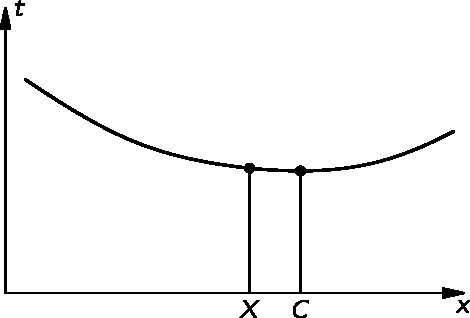
\includegraphics[width=0.7\linewidth]{fyz_fig283.pdf}
      \caption{Nejkratší čas odpovídá bodu \(C\)ale přilehlé body odpovídají přibližně stejnému času
               (\cite[s.~349]{Feynman01})}
      \label{fyz:fig283}
    \end{figure}
    Náš způsob, jak najít hledaný zákon, bude takový, že budeme uvažovat velmi malou změnu polohy a 
    budeme požadovat, aby se čas v podstatě neměnil. (Samozřejmě infinitezimální změna druhého řádu 
    tam bude; měli bychom mít kladný přírůstek času pro posunutí v obou směrech od \(C\)) Vezmeme 
    si tedy blízký bod \(X\) a vypočítáme, jak dlouhý čas bude potřebný na cestu z \(A\) do \(B\) 
    po obou drahách a porovnáme novou dráhu se starou. To lze provést velmi snadno. Chceme, 
    samozřejmě, aby rozdíl byl téměř nulový, když vzdálenost \(XC\) je krátká. Podívejme se nejprve 
    na dráhu, která vede po zemi. Nakreslíme-li si kolmici \(XE\) vidíme, že tato dráha je kratší o 
    délku \(EC\). Řekněme, že tím získáváme, neboť nemusíme běžet tuto vzdálenost. Na druhé straně, 
    nakreslíme-li si odpovídající kolmici \(CF\), vidíme, že ve vodě musíme překonat vzdálenost 
    \(XF\), a to je to, co ztrácíme. Nebo, co se týká času, získáme čas potřebný k překonání 
    vzdálenosti \(EC\), ale ztratíme čas, jenž byl potřebný na překonání vzdálenosti \(XF\). Tyto 
    dva časy si musí být rovny, neboť v prvním přiblížení se čas nesmí měnit. Za předpokladu, že 
    rychlost ve vodě je \(\frac{1}{n}\)-krát tak velká jako rychlost ve vzduchu, musíme mít
    \begin{equation}\label{fyz:eq355}
      EC = n\cdot XF.
    \end{equation}
    Vidíme, že máme-li správný bod, pak
    \begin{equation*}
      XC\sin EXC = n\cdot XC\sin XCF.
    \end{equation*}
    Dělíme-li obě strany společnou délkou přepony \(XC\) a všimneme-li si, že
    \begin{equation*}
      EXC = ECN = \alpha_1 \qquad \text{a} \qquad XCF = BCN' = \alpha_2,
    \end{equation*}
    máme
    \begin{equation}\label{fyz:eq356}
      \sin\alpha_1 = n\cdot\sin\alpha_2.
    \end{equation}
    
    Zjistili jsme, že k tomu, aby bylo možné se dostat z jednoho bodu do druhého za nejkratší dobu, 
    musí světlo dopadat pod takovým úhlem, aby poměr sinů úhlů \(\alpha_1\) a \(\alpha_2\), byl 
    roven poměru rychlostí v obou prostředích rovnému \(n\).

  \section{Použití Fermatova principu}\label{fyz:IchapXXVIsecIV}
    Nyní uvažujme o některých zajímavých důsledcích principu nejkratšího času. Prvním z nich je 
    \textbf{princip reciprocity} (princip obrácení světelného paprsku). Když jsme pro přechod z 
    \(A\) do \(B\) našli dráhu s nejmenším časem, pak pro přechod v opačném směru (za předpokladu, 
    že se světlo šíří stejnou rychlostí v každém směru) bude nejmenšímu času odpovídat táž dráha. 
    Proto, když lze světlo vyslat po jedné dráze jedním směrem, lze je po ní poslat i opačným 
    směrem.
    
    \begin{figure}[ht!] %\ref{fyz:fig284}
      \centering
      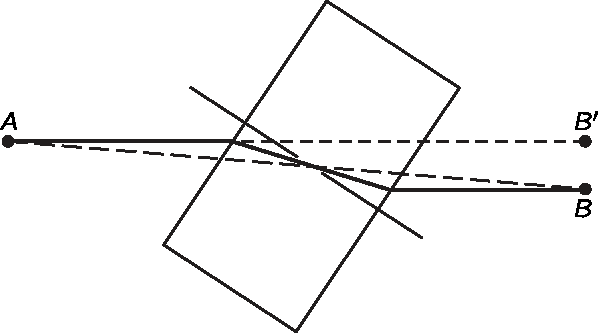
\includegraphics[width=0.9\linewidth]{fyz_fig284.pdf}
      \caption{Posunutí světelného paprsku při průchodu průhlednou destičkou
               (\cite[s.~350]{Feynman01})}
      \label{fyz:fig284}
    \end{figure}

    Zajímavým příkladem je skleněný kvádr s rovinnými rovnoběžnými stěnami, postaveny do cesty 
    světelnému paprsku pod nějakým úhlem. Světlo při průchodu kvádrem z bodu \(A\) do bodu \(B\) 
    (obr. \ref{fyz:fig284}) neprochází po přímce, ale zkracuje čas potřebný k průchodu kvádrem tím, 
    že si zmenšuje úhel náklonu v kvádru, i když tím něco ztrácí ve vzduchu. Paprsek se prostě 
    paralelně posune, neboť úhly, pod kterými světlo vniká dovnitř a zase vychází ven, jsou stejné.
    
    \begin{figure}[ht!] %\ref{fyz:fig285}
      \centering
      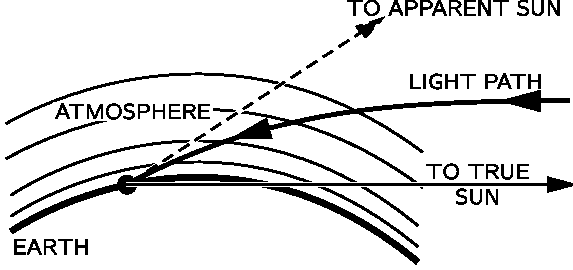
\includegraphics[width=0.9\linewidth]{fyz_fig285.pdf}
      \caption{U obzoru se Slunce zdá o 1/2stupně výž než skutečně je 
               (\cite[s.~350]{Feynman01})}
      \label{fyz:fig285}
    \end{figure}
    
    Třetím zajímavým jevem je skutečnost, že když vidíme Slunce zapadat, je vlastně už pod obzorem! 
    Není to tak, že by se zdálo být pod obzorem, ale skutečně pod ním je (obr. \ref{fyz:fig285}). 
    Zemská atmosféra je nahoře řídká a dole hustá. Sluneční světlo letí vzduchem pomaleji než ve 
    vakuu, a proto se může do bodu \(S\) za obzorem dostat rychleji, když se místo toho, aby letělo 
    po přímce, vyhne hustým oblastem, a pak je proletí pod strmějším úhlem. Když se zdá, že Slunce 
    teprve zapadá pod obzor, ve skutečnosti je už dost hluboko pod ním. Jiným příkladem tohoto jevu 
    je zrcadlení, které lze často vidět při pohybu na sluncem rozpálených silnicích. Na silnici je 
    vidět „voda“, ale když se k tomu místu dostaneme, silnice je suchá jako poušť! Tento jev 
    nastává takto: To, co ve skutečnosti vidíme, je obloha „zrcadlící“ se na silnici - světlo z 
    oblohy dopadající na silnici může skončit v našem oku, jak je to znázorněno na obr. 
    \ref{fyz:fig286}. Proč? Vzduch těsně nad silnicí je velmi horký, ale výš je chladnější. Horký 
    vzduch se více rozpíná než studený, je řidší a rychlost světla je v něm méně zpomalena. Lze 
    říci, že světlo se šíří rychleji v teplých oblastech než ve studených. Proto světlo místo toho, 
    aby se rozhodlo proletět po přímé dráze, volí dráhu s nejkratším časem. Po ní se pohybuje po 
    určitou dobu v řidším vzduchu rychleji, aby ušetřilo čas. Může tedy letět po křivočaré dráze.
    
    \begin{figure}[ht!] %\ref{fyz:fig286}
      \centering
      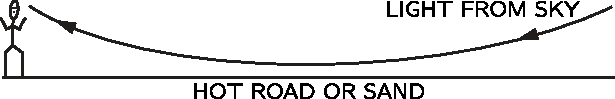
\includegraphics[width=0.9\linewidth]{fyz_fig286.pdf}
      \caption{Fata morgána
               (\cite[s.~351]{Feynman01})}
      \label{fyz:fig286}
    \end{figure}

    Jako další důležitý příklad principu nejkratšího času předpokládejme, že chceme připravit 
    situaci, aby se všechno světlo, jež vychází z jednoho bodu \(P\), znovu soustředilo v bodě 
    \(P'\) (obr. \ref{fyz:fig287}). To samozřejmě znamená, že světlo může jít z \(P\) do \(P'\) po 
    přímce. Dobře, to je v pořádku. Ale jak můžeme zabezpečit, aby nejen světlo, které jde po 
    přímce, ale i světlo vycházející z \(P\) směrem do \(Q\) také skončilo v \(P'\)? Chceme 
    soustředit všechno světlo v bodě, který nazýváme \textbf{ohniskem}. Jak? Jde-li světlo vždy po 
    dráze s nejkratším časem, určitě nebude chtít jít po všech ostatních dráhách. Jediný způsob, 
    jak se může světlo dokonale uspokojit s tím, že půjde po více sousedních dráhách, je, že jejich 
    časy si budou rovny! Jinak si vybere tu s nejkratším časem. Proto problém sestrojit takové 
    soustřeďující zařízení spočívá pouze v tom, jak zařídit, aby časy pro všechny různé dráhy byly 
    stejné!
    
    \begin{figure}[ht!] %\ref{fyz:fig287}
      \centering
      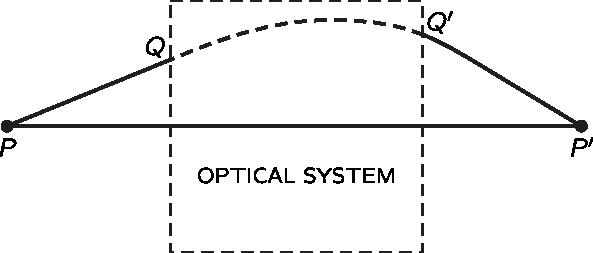
\includegraphics[width=0.7\linewidth]{fyz_fig287.pdf}
      \caption{Optická \uv{černá skříňka}
               (\cite[s.~351]{Feynman01})}
      \label{fyz:fig287}
    \end{figure}

    To lze snadno provést. Předpokládejme, že máme kus skla, jímž světlo prochází pomaleji než 
    vzduchem (obr. \ref{fyz:fig288}). Nyní si vezmeme paprsek, jenž letí vzduchem po dráze 
    \(PQP'\). Je to delší dráha než z \(P\) přímo do \(P'\) a bezpochyby jí náleží delší čas. 
    Kdybychom ale paprsku vložili do cesty kousek skla potřebné tloušťky (později si ukážeme jaké), 
    může se tak přesně vykompenzovat zbývající čas, o který se na své cestě zpozdí světlo letící 
    pod nějakým úhlem! Tak můžeme zařídit, aby čas potřebný pro světlo letící po přímce byl stejný 
    jako čas potřebný pro světlo letící po dráze \(PQP'\). Podobně, dráha paprsku \(PRR'P'\), jenž 
    je částečně odkloněn, není sice tak dlouhá jako \(PQP'\) a nepotřebujeme kompenzovat tolik času 
    jako pro paprsek letící po přímce, ale přece je třeba něco vykompenzovat. Nakonec skončíme s 
    kouskem skla, jež má tvar jako na obr. \ref{fyz:fig288}. Při takovém tvaru všechno světlo, jež 
    vychází z \(P\) dojde do \(P'\)! Samozřejmě, to dobře známe a takové zařízení nazýváme 
    \textbf{spojnou čočkou}. V další kapitole si vypočítáme, jaký tvar musí mít čočka, aby dokonale 
    soustřeďovala paprsky.

    \begin{figure}[ht!] %\ref{fyz:fig288}
      \centering
      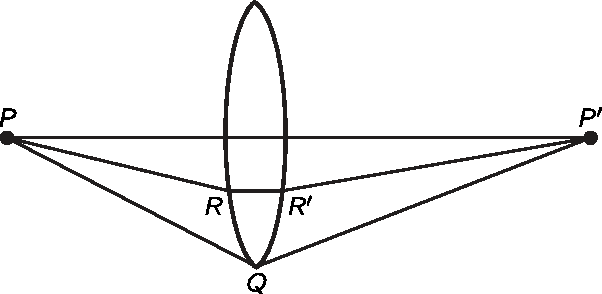
\includegraphics[width=0.7\linewidth]{fyz_fig288.pdf}
      \caption{Zaosřující optická soustava
               (\cite[s.~351]{Feynman01})}
      \label{fyz:fig288}
    \end{figure}

    Vezmeme si další příklad: předpokládejme, že chceme sestavit zrcadla tak, aby světlo z bodu 
    \(P\) šlo vždy do bodu \(P'\) (obr. \ref{fyz:fig289}). Kdyby světlo letělo z bodu \(P\) k 
    zrcadlu a odrazilo se do bodu \(P'\) po jakékoliv dráze, všechny časy, odpovídající různým 
    dráhám, musí být stejné. Světlo tady vždy prochází vzduchem, takže čas a vzdálenost jsou si 
    úměrné. Proto výrok, že všechny časy jsou stejné, znamená totéž jako výrok, že celková 
    vzdálenost je stejná. Součet dvou vzdáleností \(r_1\) a \(r_2\), musí být tedy konstantní. 
    \textbf{Elipsa} je křivka, která má tu vlastnost, že součet vzdáleností každého jejího bodu od 
    dvou daných bodů je konstantní, takže si můžeme být jisti, že se světlo z jednoho ohniska 
    dostane do druhého.
    
    \begin{figure}[ht!] %\ref{fyz:fig289}
      \centering
      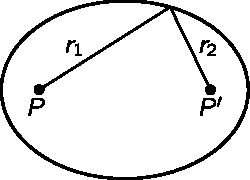
\includegraphics[width=0.5\linewidth]{fyz_fig289.pdf}
      \caption{Eliptické zrcadlo
               (\cite[s.~351]{Feynman01})}
      \label{fyz:fig289}
    \end{figure}

    Stejný princip se uplatňuje při zachycování světla hvězdy. Velký pětimetrový teleskop v 
    observatoři na Mt. Palomar je založen na tomto principu: Představme si hvězdu vzdálenou 
    miliardy kilometrů. Chceme způsobit, aby se všechno světlo, které z ní přichází, soustředilo do 
    jednoho bodu. Samozřejmě, že si nemůžeme nakreslit dráhy paprsků až po hvězdu, ale přece se 
    chceme přesvědčit, zda jsou časy stejné. Samozřejmě víme, že když různé paprsky přiletěly na 
    nějakou rovinu \(KK'\), na ně kolmou, jsou v této rovině všechny časy stejné (obr. 
    \ref{fyz:fig290}). Proto musí paprsky letět dále k zrcadlu a pokračovat v cestě do \(P'\) za 
    stejný čas, tj. musíme najít takovou křivku, pro niž součet vzdáleností \(XX' + X'P'\) je 
    konstanta, bez ohledu na to, kde zvolíme \(X\). Snadný způsob, jak to lze najít, spočívá v 
    prodloužení čáry \(XX'\) po rovinu \(LL'\). Sestrojíme-li nyní takovou křivku, že \(A'A" = 
    A'P'\), \(B'B" = B'P'\), \(C'C" = C'P'\) atd., bude to hledaná křivka. Samozřejmě platí, že 
    \(AA' + A'P' = AA' + A'A"\), a to bude konstanta. Naše křivka je tedy množinou všech bodů 
    \emph{ekvidistantních} od dané přímky a daného bodu. Takovou křivku nazýváme parabola, zrcadlo 
    má tvar \textbf{paraboly}.

    \begin{figure}[ht!] %\ref{fyz:fig290}
      \centering
      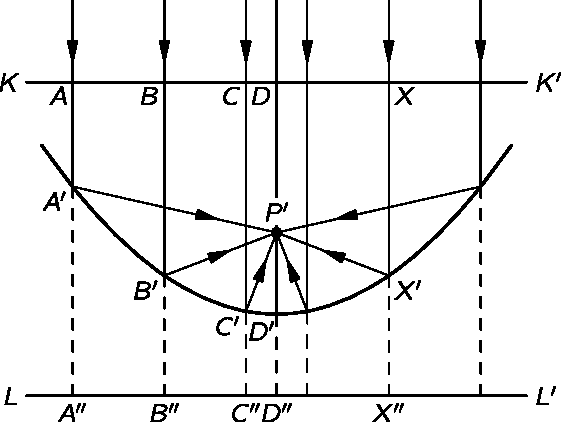
\includegraphics[width=0.8\linewidth]{fyz_fig290.pdf}
      \caption{Parabolické zrcadlo
               (\cite[s.~352]{Feynman01})}
      \label{fyz:fig290}
    \end{figure}

    Uvedené příklady slouží pro ilustraci principu, podle něhož lze projektovat optická zařízení. 
    Přesné křivky lze vypočítat pomocí principu, že k vytvoření dokonalého ohniska musí být časy 
    potřebné k průletu dráhy rovny pro všechny paprsky, a musí být zároveň kratší než časy pro 
    jakoukoliv jinou blízkou dráhu.
    
    Tato ohnisková optická zařízení budeme probírat v následující kapitole; nyní si proveďme 
    diskuzi dalšího rozvoje teorie. Rozpracuje-li se nový teoretický princip, jako je princip 
    nejkratšího času, může nás to zpočátku svádět k tomu, abychom řekli: \uv{Dobře, to je velmi 
    pěkné,je to úžasné, ale otázkou je, zda nám to vůbec pomohlo v našem chápání fyziky.} Někdo nám 
    může říct: \uv{Ano, podívejte se, kolik věcí umíme nyní pochopit!} Jiný může namítnout: \uv{Ale 
    já také rozumím principu zrcadla. Potřebuji takovou křivku, aby každá tečná rovina vytvářela s 
    dvěma paprsky stejné úhly. Umím si také vypočítat čočku, neboť každý paprsek, jenž jí prochází, 
    se odklání o úhel daný Snellovým zákonem.} Je jasné, že výrok o nejkratším čase a výrok, že 
    úhly jsou si při odrazu rovny a siny úhlů při lomu jsou si úměrné, jsou rovnocenné výroky. Je 
    to tedy jen pouhá filozofická otázka nebo otázka krásy? Argumenty mohou potvrzovat obojí. 
    
    Avšak důležitost účinného principu spočívá v tom, že \emph{předpovídá nové věci}. 
    
    Snadno lze ukázat, že existuje řada věcí, na něž můžeme usuzovat z Fermatova principu. Nejprve 
    předpokládejme, že máme tři prostředí - sklo, vodu a vzduch; provádíme experiment s lomem 
    světla a měříme index \(n\) pro přechod z jednoho média do druhého. Index lomu na rozhraní mezi 
    vzduchem (1) a vodou (2) označíme \(n_{12}\); index lomu na rozhraní mezi vzduchem (1) a sklem 
    (3) označíme \(n_{13}\). Kdybychom měřili index lomu mezi vodou a sklem, našli bychom další 
    index lomu, který označíme \(n_{23}\). A priori však není žádný důvod, proč by mezi \(n_{12}\), 
    \(n_{13}\) a \(n_{23}\) měla být jakákoliv souvislost. Na druhé straně podle myšlenky 
    nejkratšího času existuje mezi nimi určitý vztah. Index \(n_{12}\) je roven poměru dvou veličin 
    - rychlosti světla ve vzduchu a rychlosti světla ve vodě; \(n_{13}\) je roven poměru rychlostí 
    ve vzduchu a ve skle, \(n_{23}\) je roven poměru rychlostí ve vodě a skle. Proto rozšíříme 
    zlomek rychlostí ve vzduchu v a dostaneme
    \begin{equation}\label{fyz:eq357}
      n_{23} = \frac{v_2}{v_3} = \dfrac{\dfrac{v_1}{v_3}}{\dfrac{v_1}{v_2}} = \frac{n_{13}}{n_{12}}.
    \end{equation}
    
    Jinými slovy, předpovídáme, že index pro nový pár materiálů lze získat z indexů pro jednotlivé 
    materiály vzhledem ke vzduchu nebo k vakuu. Takže, změříme-li rychlost světla ve všech 
    materiálech, jmenovitě jejich indexy vzhledem k vakuu, označené jako \(n_i\), (\(n_1\) je poměr 
    rychlosti ve vzduchu a ve vakuu atd.), dostaneme jednoduchý vzorec. Index lomu pro jakékoliv 
    dva materiály \(i\) a \(j\) je
    \begin{equation}\label{fyz:eq358}
      n_{ij} = \frac{v_i}{v_j} = \frac{n_j}{n_i}.
    \end{equation}
    
    Předpověď takového druhu bychom nebyli schopni udělat, kdybychom vycházeli jen ze Snellova 
    zákona\footnote{Takovou předpověď lze provést pomocí Snellova zákona, uděláme-li dodatečný 
    předpoklad, že položením vrstvy jedné látky na povrch druhé látky se úhel lomu v druhé látce 
    nezmění.}. Ale tato předpověď je pravdivá.
    
    Vztah (\ref{fyz:eq357}) byl znám velmi dávno a byl silným argumentem pro princip nejkratšího 
    času.
    
    Dalším argumentem pro princip nejkratšího času a další předpovědí je, že změříme-li rychlost 
    světla ve vodě, bude menší než ve vzduchu. Toto je předpověď zcela jiného typu. Je přímo 
    skvělá, neboť dosud jsme měřili pouze úhly. Máme zde teoretickou předpověď, která se velmi liší 
    od pozorování, z nichž Fermat vydedukoval myšlenku nejkratšího času. Ukazuje se, že rychlost ve 
    vodě je skutečně menší než rychlost ve vzduchu právě o tolik, kolik je potřebné k tomu, abychom 
    dostali správný index lomu!
    
  \section{Přesnější formulace Fermatova principu}\label{fyz:IchapXXVIsecV}
    Princip nejkratšího času musíme formulovat o něco přesněji než jsme zatím uvedli. Dosud jsme ho 
    formulovali nesprávně. Nesprávně se mu říká princip nejkratšího času, i my jsme ho tak nazývali 
    pro pohodlnost, ale nyní si musíme uvést jeho přesné znění. Předpokládejme, že máme zrcadlo, 
    jaké je na obr. \ref{fyz:fig281}. Co způsobí, že světlo „ví“, že má jít k zrcadlu? Dráha 
    nejkratšího času je \(AB\), to je jasné. Někdo by mohl říct: „někdy je to nejdelší čas.“ 
    Nejdelší čas to určitě není, neboť zakřivené dráze náleží ještě delší čas! Správné tvrzení je 
    takové: Paprsek jdoucí po určité dráze má tu vlastnost, že uděláme-li malou změnu (např. 
    posunutí o jedno procento) paprsku jakýmkoliv způsobem, řekněme v místě, v němž dopadá na 
    zrcadlo, nebo v tvaru křivky nebo jakoukoli jinou, v prvním přiblížení se čas nezmění; čas se 
    změní jen v přiblížení druhého řádu. Jinými slovy, princip spočívá v tom, že světlo jde po 
    dráze tak, že v blízkosti je mnoho jiných drah, po nichž mu cesta trvá téměř stejnou dobu.
    
    Další problém s principem nejkratšího času neumí nikdy strávit lidé, kteří nemají rádi takový 
    druh teorie. Pomocí Snellovy teorie umíme světlo „chápat“. Světlo se šíří, vidí povrch, změní 
    směr, neboť se s ním na povrchu něco stane. Myšlenku příčinnosti, postup od bodu k bodu, lze 
    snadno pochopit, ale princip nejkratšího časuje zcela jiný filozofický princip o tom, jak 
    pracuje příroda. Místo toho, aby říkal, že je to kauzální záležitost, že když něco uděláme, 
    něco dalšího se stane atd., říká toto: my aranžujeme situaci a světlo se rozhoduje, který čas 
    je nejkratší nebo extrémní a podle toho si vybere dráhu. Ale jak to dělá, jak jí najde? Cožpak 
    „cítí“ blízké dráhy a vzájemně je porovnává?
    
    \begin{figure}[ht!] %\ref{fyz:fig291}
      \centering
      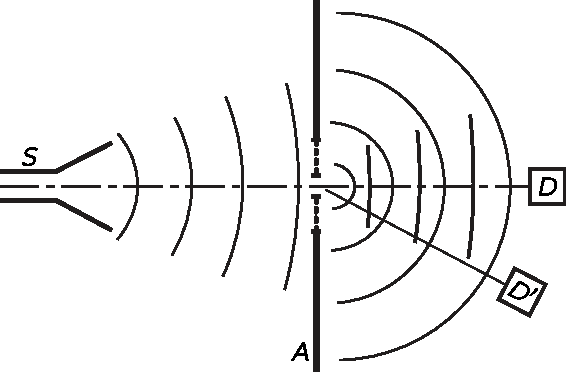
\includegraphics[width=0.7\linewidth]{fyz_fig291.pdf}
      \caption{Průchod rádiových vln úzkou štěrbinou
               (\cite[s.~354]{Feynman01})}
      \label{fyz:fig291}
    \end{figure}
    
    Odpověď zní v jistém smyslu ano. Je to vlastnost světla, která není známá v geometrické optice 
    a která spočívá v myšlence \emph{vlnové délky}, vlnová délka nám přibližně řekne, jak daleko 
    musí světlo „očichat“ dráhu, aby si ji zkontrolovalo. Při velkých rozměrech zařízení lze tento 
    efekt velmi obtížně ukázat pomocí světla, neboť jeho vlnové délky jsou hrozně krátké, ale u 
    rádiových vln, řekněme 3centimetrových, jsou vzdálenosti, jež rádiové vlny kontrolují, větší. 
    Máme-li zdroj rádiových vln, detektor a štěrbinu, jako na obr. \ref{fyz:fig291}, je samozřejmé, 
    že paprsky jdou z \(S\) do \(D\), neboť to je přímka a přivřeme-li štěrbinu - ještě stále skrz 
    ní procházejí, což je v pořádku. Přemístíme-li však nyní detektor na stranu do \(D'\), vlny 
    nepůjdou z \(S\) do \(D'\) širokou štěrbinou, neboť si zkontrolují několik přilehlých drah a 
    řeknou si: „Ne, příteli, ty všechny odpovídají různým časům.“ Když ale \emph{znemožníme} záření 
    kontrolovat dráhy tím, že štěrbinu přivřeme až na úplně úzkou mezeru, zůstane volná pouze jedna 
    dráha a záření ji použije! U úzké štěrbiny dopadne na \(D'\) víc záření než u široké!
    
    Totéž lze provésti se světlem, ale obtížně to lze ukázat u velkých rozměrů. Tento efekt lze 
    pozorovat za velmi jednoduchých podmínek: Najděte ostré světlo, řekněme velmi vzdálenou 
    pouliční lampu s čirou žárovkou nebo odraz slunce na zaobleném nárazníku auta. Pak si dejme dva 
    prsty před jedno oko tak, abychom viděli štěrbinou mezi nimi a štěrbinu pomalu opatrně 
    zmenšujeme. Uvidíme, že obraz lampy, který byl předtím malou tečku, se začne prodlužovat a 
    dokonce se roztáhne do dlouhé čáry. Důvodem je, že prsty jsou velmi blízko sebe a světlo, jež 
    by mělo přicházet po přímce, se rozšíří na celý úhel, takže vchází do oka z různých směrů. 
    Pokud jste velmi pozorní, uvidíte možná vedlejší maxima a množství proužků při okrajích. Navíc, 
    celý obraz je zbarvený. To vše si časem vysvětlíme, ale nyní je to ukázka toho, že světlo se ne 
    vždy šíří přímočaře, a přitom snadno proveditelná.
    
  \section{Jak tomu rozumět}\label{fyz:IchapXXVIsecVI}
    Nakonec uvedeme velmi hrubý pohled na to, co se skutečně děje, jak celá věc probíhá podle toho, 
    o čem dnes věříme, že je správné, kvantově-dynamicky přesné hledisko, ale samozřejmě, popsané 
    jen kvalitativně. Sledujeme-li světlo z \(A\) do \(B\) na obr. \ref{fyz:fig281}, zjistíme, že 
    se nezdá, že by mělo podobu vln. Spíš se zdá, že se paprsky skládají z fotonů a ty skutečně 
    způsobují cvaknutí ve fotočítači, pokud ho použijeme. Jasnost světla je úměrná průměrnému 
    množství fotonů přicházejících za sekundu a to, co počítáme, je pravděpodobnost, že se foton 
    dostane z bodu \(A\) do bodu \(B\) řekněme tím, že narazí na zrcadlo. Zákon pro takovou 
    pravděpodobnost je následující a velmi podivný. Vezmeme si kteroukoliv dráhu a zjistíme k ní 
    náležící čas. Pak utvoříme komplexní číslo nebo nakreslíme vektor \(\varrho e^{i\vartheta}\), 
    kde úhel \(\vartheta\) je úměrný zjištěnému času. Počet obrátek za sekundu je frekvence 
    světla. Nyní vezmeme jinou dráhu, jíž náleží jiný čas, takže její vektor se otáčí s jiným 
    úhlem, jenž je stále úměrný času. Vezměme si všechny možné dráhy a sčítejme jejich všechny malé 
    vektory. Odpověď zní: Pravděpodobnost příchodu fotonu je úměrná druhé mocnině délky výsledného 
    vektoru od začátku do konce!
    
    Ukažme si, jak z toho vyplývá princip nejkratšího času pro zrcadlo. Uvažujme všechny paprsky, 
    všechny možné dráhy \(ADB\), \(AEB\), \(ACB\) atd. zobrazené na obr. \ref{fyz:fig292}. Dráha 
    \(ADB\) vytvoří určitý příspěvek, ale další dráze \(AEB\) přísluší zcela jiný čas, takže úhel 
    úje zcela jiný. Řekněme, že bodu \(C\) odpovídá minimální čas, a změníme-li malinko dráhu, čas 
    se nezmění. Chvíli se tedy časy mění a pak, když se blížíme k bodu \(C\), se začínají časy 
    měnit méně a méně (obr. \ref{fyz:fig292}). Takže šipky, jež máme sčítat, mají v okolí \(C\) 
    téměř stejný úhel a pak se čas začne znovu postupně zvětšovat a fáze se začnou točit na druhou 
    stranu. Nakonec máme docela hustý uzel. Celková pravděpodobnost je rovna druhé mocnině celkové 
    vzdálenosti od jednoho konce do druhého. \emph{Téměř všechna nahromaděná pravděpodobnost se 
    nachází v oblasti, kde mají všechny šipky stejný směr} (nebo stejnou fázi). Všechny příspěvky 
    od drah, jež mají velmi odlišné časy při změně dráhy, se navzájem ruší, neboť příslušné vektory 
    mají různé směry. To je důvod, proč zrcadlo odráží téměř stejně, zakryjeme-li jeho vzdálené 
    části, neboť všechno, co jsme tím udělali, je, že jsme odstranili části diagramu uvnitř 
    spirálových konců a to způsobí jen velmi malou změnu světla. To je tedy vztah mezi fotonovým 
    obrazem s pravděpodobností dopadu závisející na nahromadění šipek a mezi principem nejkratšího 
    času.
    
    \begin{figure}[ht!] %\ref{fyz:fig292}
      \centering
      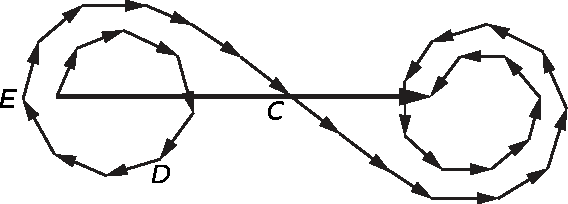
\includegraphics[width=0.7\linewidth]{fyz_fig292.pdf}
      \caption{Sčítání amplitud pravděpodobností pro mnoho sousedních drah
               (\cite[s.~355]{Feynman01})}
      \label{fyz:fig292}
    \end{figure}

  \section{Příklady a cvičení}\label{fyz:IchapXXVIsecVII}
  
%} %tikzset
%---------------------------------------------------------------------------------------------------
\printbibliography[title={Seznam literatury}, heading=subbibliography]
\addcontentsline{toc}{section}{Seznam literatury}